% IEEE Paper Template for US-LETTER Page Size (V1)
% Sample Conference Paper using IEEE LaTeX style file for US-LETTER pagesize.
% Copyright (C) 2006-2008 Causal Productions Pty Ltd.
% Permission is granted to distribute and revise this file provided that
% this header remains intact.
%
% REVISION HISTORY
% 20080211 changed some space characters in the title-author block
%
% \documentclass[10pt,conference,letterpaper]{IEEEtran}
% \usepackage{times,amsmath,epsfig}
% \usepackage[utf8]{inputenc}
% \usepackage[usenames,dvipsnames]{color}
% \usepackage{amssymb}

\documentclass[a4paper,english]{llncs}
\usepackage[T1]{fontenc}
\usepackage[latin9]{inputenc}
\usepackage{lmodern}
\usepackage{float}
\usepackage{slashed}
\usepackage{graphicx}
\usepackage{fixltx2e}
\usepackage{amsmath}
\usepackage{epstopdf}
\usepackage{url}
\usepackage{seqsplit} % for splitting very long variable names
\usepackage[dvipsnames]{xcolor}
\usepackage{listings}

\hyphenation{bio-ban-kers}
\hyphenation{Bio-bank-Cloud}

\newcommand\YAMLcolonstyle{\color{black}}
\newcommand\YAMLkeystyle{\color{blue}}
\newcommand\YAMLvaluestyle{\color{black}}

% \newcommand\language@yaml{yaml}
% 
% \expandafter\expandafter\expandafter\lstdefinelanguage
% \expandafter{\language@yaml}
% {
%   keywords={name,ec2,type,region,cookbooks,groups,size,recipes,github,branch},
%   keywordstyle=\color{blue}\bfseries,
%   basicstyle=\color{black},                                 % assuming a key comes first
%   sensitive=false,
%   comment=[l]{\#},
%   morecomment=[s]{/*}{*/},
%   commentstyle=\color{purple}\ttfamily,
%   stringstyle=\YAMLvaluestyle\ttfamily,
%   moredelim=[l][\color{orange}]{\&},
%   moredelim=[l][\color{magenta}]{*},   % switch to value style at :
%   literate =    {---}{{\ProcessThreeDashes}}3
%                 {>}{{\textcolor{red}\textgreater}}1     
%                 {|}{{\textcolor{red}\textbar}}1 
%                 {\ -\ }{{\mdseries\ -\ }}3,
% }
% 
% % switch to key style at EOL
% \lst@AddToHook{EveryLine}{\ifx\lst@language\language@yaml\YAMLkeystyle\fi}
% % \makeatother
% 
% \newcommand\ProcessThreeDashes{\llap{\color{cyan}\mdseries-{-}-}}
% 
% \usepackage{hyperref}
% \newcommand\fnurl[2]{%
% \footnote{\label{#1}\href{#2}{#2}}%
% }
% 



\makeatletter
\raggedbottom % remove unwanted space between paragraphs 

%%%%%%%%%%%%%%%%%%%%%%%%%%%%%% LyX specific LaTeX commands.
\pdfpageheight\paperheight
\pdfpagewidth\paperwidth

\floatstyle{ruled}
\newfloat{algorithm}{tbp}{loa}
\providecommand{\algorithmname}{Algorithm}
\floatname{algorithm}{\protect\algorithmname}

%%%%%%%%%%%%%%%%%%%%%%%%%%%%%% User specified LaTeX commands.
\usepackage{paralist}
\usepackage[noend]{algorithm,algcompatible,algpseudocode}
\usepackage{amssymb} % for symbols 
\usepackage{caption} % algorthm is a float and does not split. use caption instead
% \usepackage{subcaption}
\usepackage{etoolbox}\AtBeginEnvironment{algorithmic}{\footnotesize}
%\algsetup{linenosize=\small}
\usepackage{subfig}
\usepackage[T1]{fontenc}
\usepackage{mwe}    % loads »blindtext« and »graphicx«

\makeatother
\algblockdefx[NAME]{StartTransaction}{EndTransaction}
[1]{\textbf{begin transaction} \textbf{#1}}{\textbf{commit transaction}}
\algrenewcommand\alglinenumber[1]{\footnotesize #1:}

\usepackage{babel}
\usepackage{cite}
\usepackage{amssymb}% http://ctan.org/pkg/amssymb
\usepackage{pifont}% http://ctan.org/pkg/pifont
\newcommand{\cmark}{\ding{51}}%
\newcommand{\xmark}{\ding{53}}%

\title{BiobankCloud: a Platform for the Secure Storage, Sharing, and Processing of Large Biomedical Data Sets}

\author{Alysson Bessani\inst{5}, J\"{o}rgen Brandt\inst{2}, Marc Bux\inst{2}, Vinicius Cogo\inst{5}, Lora Dimitrova\inst{4}, Jim Dowling\inst{1}, Ali Gholami\inst{1}, Kamal Hakimzadeh\inst{1}, Micheal Hummel\inst{4}, Mahmoud Ismail\inst{1}, Erwin Laure\inst{1}, Ulf Leser\inst{2}, Jan-Eric Litton\inst{3}, Roxanna Martinez\inst{3}, Salman Niazi\inst{1}, Jane Reichel\inst{6}, Karin Zimmermann\inst{4}}

\institute{KTH - Royal Institute of Technology,\\
\email{\{jdowling, gholami, mahh, maism, erwinl, smkniazi\}@kth.se}
\and
Humboldt University\\
\email{\{leser, bux, joergen.brandt\}@informatik.hu-berlin.de}
\and
Karolinska Institute\\
\email{\{Jan-Eric.Litton, Roxanna.Martinez\}@ki.se}
\and
Charite\\
\email{\{Michael.Hummel, Lora.Dimitrova, Karin.Zimmermann\}@charite.de}
\and
LaSIGE, Faculdade de Ci\^{e}ncias, Universidade de Lisboa, Portugal\\
\email{\{bessani, vielmo\}@lasige.di.fc.ul.pt}
\and
Uppsala University\\
\email{\{jane.reichel\}@jur.uu.se}
}

\newif\ifshowcomments
\showcommentstrue

\ifshowcomments
\newcommand{\mynote}[2]{\fbox{\bfseries\sffamily\scriptsize{#1}}
{\small$\blacktriangleright$\textsf{\emph{#2}}$\blacktriangleleft$}}
\else
\newcommand{\mynote}[2]{}
\fi
\newcommand{\jim}[1]{\textcolor{Red}{\mynote{Jim}{#1}}}

\begin{document}
\maketitle

\begin{abstract}
Biobanks store and catalog human biological material that is increasingly being digitized using next-generation sequencing (NGS). There is, however, a computational bottleneck, as existing software systems are not scalable and secure enough to store and process the incoming wave of genomic data from NGS machines. In the BiobankCloud project, we are building a Hadoop-based platform for the secure storage, sharing, and parallel processing of genomic data. We extended Hadoop to include support for multi-tenant studies, reduced storage requirements with erasure coding, and added support for extensible and consistent metadata. On top of Hadoop, we built a scalable scientific workflow engine featuring a proper workflow definition language focusing and simple integration and chaining of existing tools, adaptive scheduling on Apache Yarn, and support for iterative dataflows. Our platform also supports the secure sharing of data across different, distributed Hadoop clusters. The software is easily installed and comes with a provide user-friendly web interface for running, managing, and accessing data sets behind a secure 2-factor authentication. Initial tests have shown that the engine scales well to dozens of nodes. The entire system is open-source and includes pre-defined workflows for popular tasks in biomedical data analysis, such as variant identification, differential transcriptome analysis using RNA-Seq, and analysis of miRNA-Seq, and ChIP-Seq data.
\end{abstract}

%\vskip-5pt
\section{Introduction}
Biobanks store and catalog human biological material from identifiable individuals for both clinical and research purposes. Recent advances in Next-Generation Sequencing (NGS) technology has meant that there is an increasing demand to sequence the human biological material stored in Biobanks. Both research projects and clinical health-care systems use Biobanks to store samples that are sequenced using techniques from genotyping to whole-genome sequencing (WGS). Biobanks' computer systems have traditionally managed only metadata associated with samples, such as pseudo-identifiers for patients, sample collection information, study infromation, and data concerning samples. Alongside this metadata, we now increasingly need to store genomic data, which requires anything from MBs (genotyping) up to several hundred GBs (WGS) of data per sample.
The data storage requirements for large-scale WGS sequencing projects, such as the 100,000 genomes project by Genomics England, now scale to many PBs, and are so large that researchers are looking at cost-effective Big Data solutions based on commodity hardware, such as Hadoop. When data volumes grow past several TBS, traditional database technology (including sharded relational databases) is no longer viable, as more data needs to be moved from storage to compute nodes that is possible with current networking technology. The solution provided by platforms such as Hadoop is to move computation to where the data is located, exploiting the principle of \textit{data locality}. That is, jobs are parallelized across many nodes and each job loads its (large) input data primarily from disk subsystems, while network I/O is used transfer in subsequent processing and sorting steps on, typically, smaller data volumes relative to the input data size.

In this paper, we introduce BiobankCloud, an integrated platform, based on Hadoop, for the secure storage, processing, and sharing of genomic data and associated metadata. BiobankCloud is a platform-as-a-service that can be automatically deployed on public clouds, private clouds or bare-metal servers. As part of BiobankCloud, we also provide a Laboratory Information Management Service (LIMS) as software-as-a-service (SaaS). The LIMS has an integrated User Interface (UI) for authenicating/authorizing users, managing data, designing and searching for metadata, and support for running workflows and analysis jobs on Hadoop. The LIMS hides much of the complexity of the Hadoop backend, and supports multi-tenancy through first-class support for \textit{Studies}, \textit{SampleCollections} (DataSets), \textit{Samples}, and \textit{Users}.

In BiobankCloud, we have developed our own Hadoop distribution, Hadoop Open Platform-as-a-Service (Hops), with improved scalability and customizability properties, enabled by a new metadata storage system based on a distributed in-memory database.

Existing scientific workflow management systems are typically custom-built and have not been designed for data parallel processing with data locality. For performance reasons, their architectures and file formats are typically flat (monolithic). None of the main file formats in genomics (fastq, BAM/SAM, CRAM, and VCF) have support for data parallel processing because of their assumption of centralized metadata (e.g., in the file header). 
In BiobankCloud, we provide a scientific workflow management system, SaasFee, as a native YARN/Hadoop 2nd-level scheduler that provides a bridge between support for existing file formats and data parallel processing. SaasFee can both speedup workflows, such as a ??x speedup for NGS varient calling on XX machines, and scale-out to support larger clusters.
%\vskip-5pt
\section{Related work}
There are a couple of frameworks for data parallel processing of genomic data. Adam, Halvade, Seal, PigSeq, Spork?

There's the big Alvados? project in Harvard.

In security, Hadoop has support for Apache Ranger (attribute-based access control), Apache Sentry (Databases, RBAC), and Apache ?? (RBAC for REST APIs).

Nothing happening in Biobanking?


% \input{regulation}
%\vskip-5pt
\section{LIMS}

 \begin{figure}[h]
 \centering
 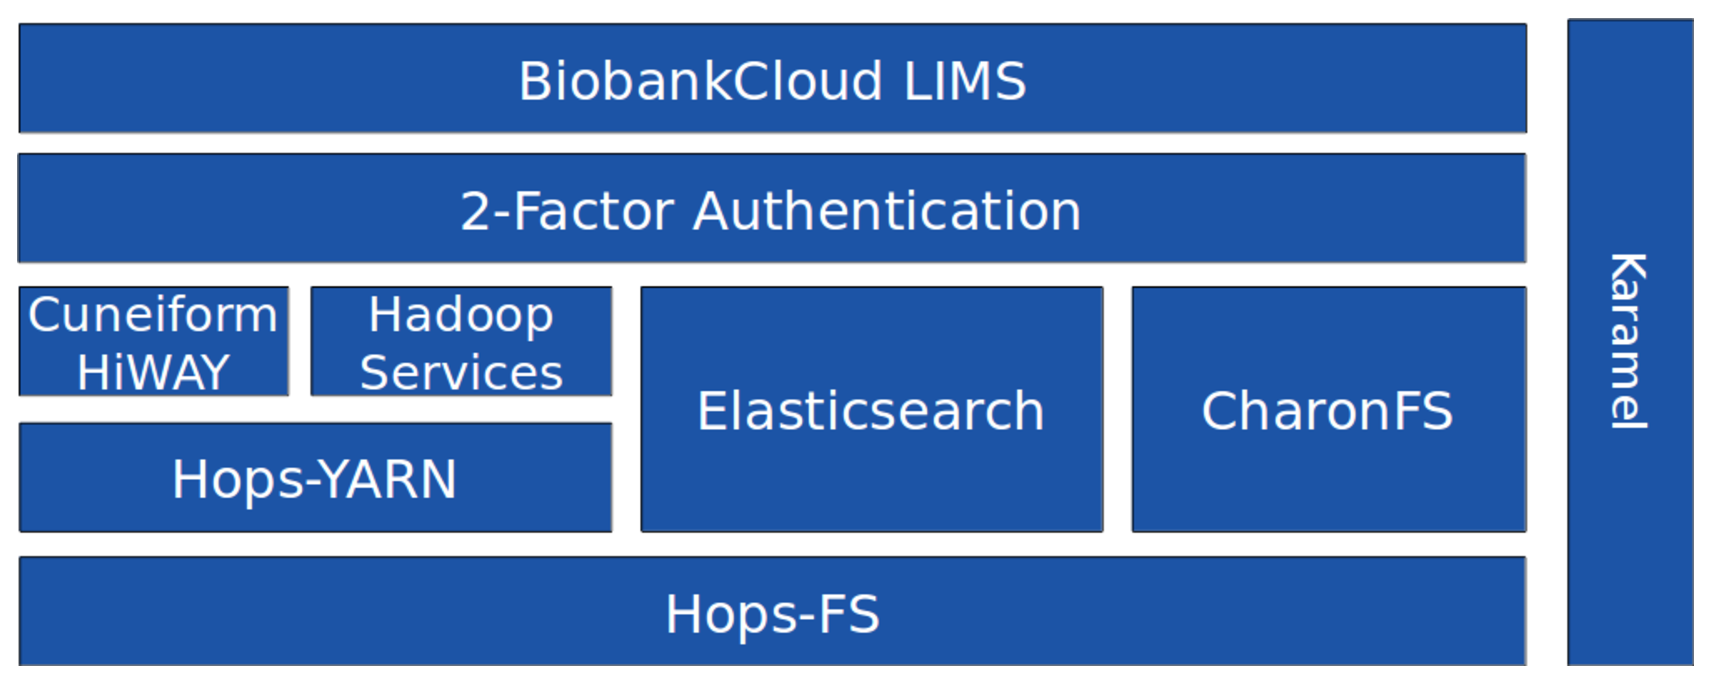
\includegraphics[scale=0.8]{./imgs/stack.eps}
 % stack.eps: 0x0 pixel, 300dpi, 0.00x0.00 cm, bb=0 -1 805 312
 \caption{BiobankCloud Architecture}
 \label{fig:lim}
\end{figure}


BiobankCloud introduces \textbf{DataSets} as a new abstraction to Hadoop, where a DataSet consists of a related group of directories, files, and extended metadata. DataSets can be indexed and searched and are the basic unit of data management in BiobankCloud; all user-generated files or directories belong to a single DataSet. In Biobanking, a sample collection would be a typical example of a DataSet.  To allow for access control of users to DataSets, which is not inherent in the DataSet concept, we introduce the notion of \textbf{Studies}. A Study is a grouping of researchers and DataSets , see figure \ref{fig:studies}. 
% The basic user roles we provide reflect the European Data Protection Directive, with a DataOwner (data controller) and a DataScientist (data processer). DataSets can be shared between Studies (when the necessary security, legal, and ethical conditions for sharing are in place).  In BiobankCloud, we use the access control mechanism of HopsFS to implement the Study- and DataSet-based authorization model. 
% Roles are defined and privileges are enforced in HopsFS.
\begin{figure}[h]
 \centering
 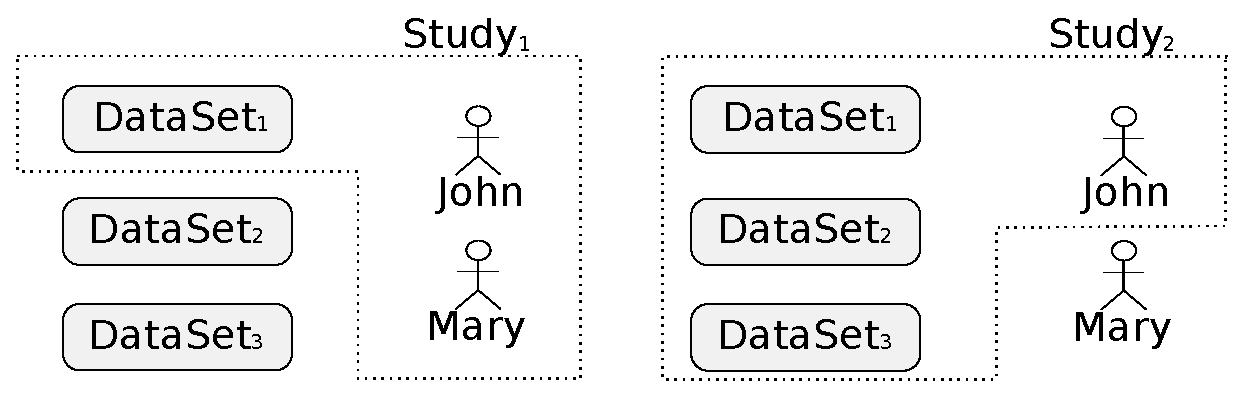
\includegraphics[scale=0.6]{./imgs/projects-as-groupings1.eps}
 % projects-as-groupings1.eps: 0x0 pixel, 300dpi, 0.00x0.00 cm, bb=0 207 582 382
\caption{Study1 has two Users and one DataSet, while Study2 has one User and three DataSets.}
\label{fig:studies}
\end{figure}

%\vskip-5pt
\section{Security Model}

The BioBankCloud environment deploys strong security features for concerns such as Confidentiality, Integrity and Non-repudiation ~\cite{BBCSEC} of data access. This includes authentication, authorization
, and auditing. The system allows defining different roles with different access privileges. In designing the system, we applied the Cloud Privacy Threat Modeling~\cite {CPTM} approach to identify the privacy requirements of processing sensitive biomedical data.



Figure \ref{fig:security} shows the different components of the employed security mechanisms. All BioBankCloud services are protected behind the firewall and only accessible through the secure interfaces over HTTPS Channels.


\begin{figure}[h]
\centering
\includegraphics[width=\textwidth]{./imgs/security.png}
% stack.eps: 0x0 pixel, 300dpi, 0.00x0.00 cm, bb=0 -1 805 312                                                                                                                                               
\caption{Security Architecture of the BiobankCloud}
\label{fig:security}
\end{figure}


\subsection{2-Factor Authentication}
 The authentication services map the person accessing the platform to a user identity. We provide two-factor authentication using smart mobile devices or Yubikey hardware tokens to support different groups of users.

\subsection {Access Control}
The accessc control component ensures authorized access to genomics data as internal objects or different services within the platform. This is accomplished through a role-based access control (RBAC) model and a data access approach using the ownership of data on the HDFS, for example, a data owner adds/revokes members to a study and assigns privileges to access the study.


\subsection{HDFS Supported Authorization}

\begin{figure}[h]
 \centering
 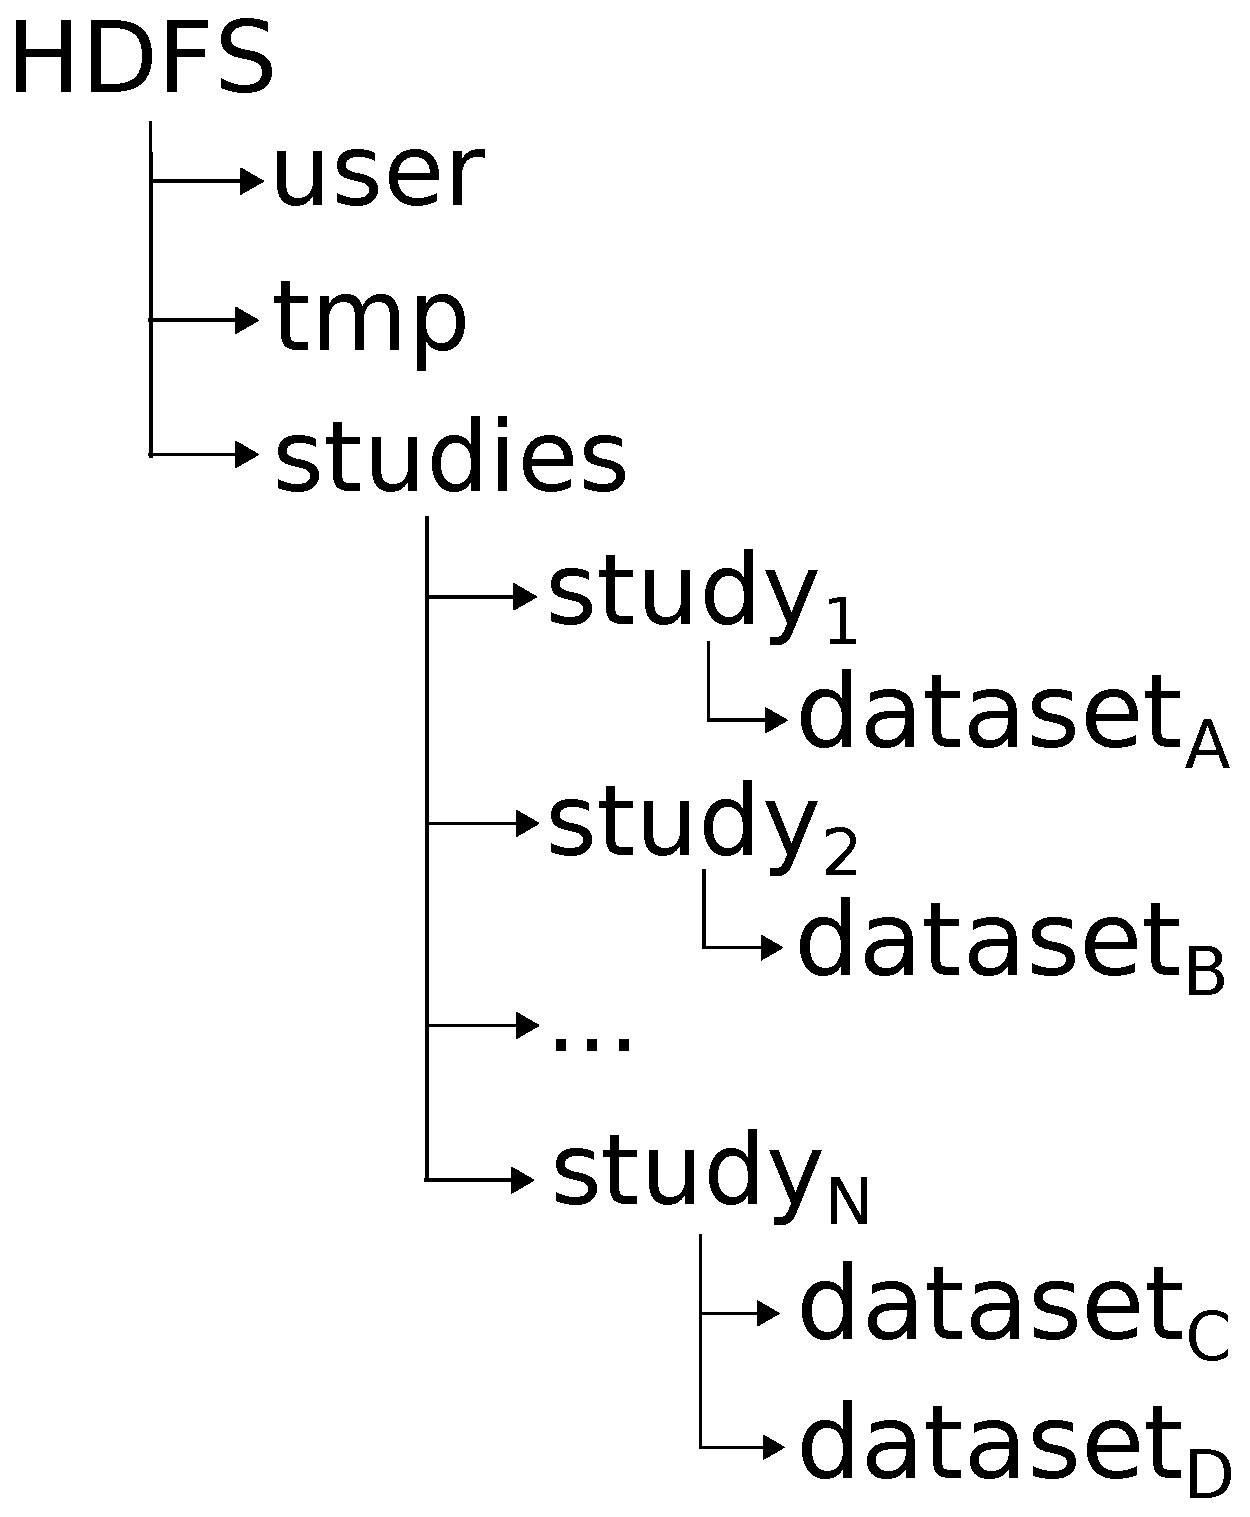
\includegraphics[scale=0.2]{./imgs/HDFS-structure.eps}
 % HDFS-structure.eps: 0x0 pixel, 300dpi, 0.00x0.00 cm, bb=0 -1 584 711
 \caption{Filesystem structure in HDFS containing Studies and DataSets.}
\end{figure}


\subsection {Auditing Service}
Finally, the auditing service enables the platform administrator or an external auditor to discover the history of accessing the platform to detect any violation to a policy. It includes several contexts \
such as role, account, study, and login audits. The secure login service assures that actions that are taken by the users are registered for tracing and auditing purposes. Each log event contains informat\
ion such as initiator, target, IP/MAC addresses, timestamp, action, and outcome.

%\vskip-5pt
\section{Hadoop Open Platform-as-a-Service (Hops)}

% Jim - 1-3 pages
We have moved metadata from the heap of a Java Virtual Machine to an in-memory, no-shared-state, distributed database, called MySQL Cluster~\cite{ronstrom2005recovery}. We ensure the consistency of the filesystem metadata by implementing serialized transactions on well-ordered operations on metadata~\cite{hops_consistency}.
We do not need Zookeeper, as we have developed a leader-election service based on the database~\cite{hopselection}.
%\vskip-5pt
\section{SAASFEE}

%one page, should include an evaluation (see Introduction)
%one paragraph on saasfee (possibly w/ img)
%one paragraph on hiway
%one paragraph on cuneiform
%one paragraph on evaluation (w/ image)

To process the vast amounts of genomic data stored in today's Biobanks, researchers have a diverse ecosystem of tools at their disposal~\cite{Pabinger2014}. Depending on the research question at hand, these tools are often used in conjunction with one another, resulting in complex and intertwined analysis pipelines. Scientific workflow management systems (SWfMSs) facilitate the design, refinement, execution, monitoring, sharing, and maintenance of such analysis pipelines. SAASFEE~\cite{vldb_demo} is a SWfMS that supports the scalable execution of arbitrarily complex workflows. It encompasses the functional workflow language Cuneiform as well as Hi-WAY, a higher-level scheduler for Hadoop YARN.

Paragraph on Cuneiform~\cite{cuneiform} (ToDo Joergen)

Hi-WAY is a higher-level scheduler for executing scientific workflows on Hadoop YARN. It provides a selection of established scheduling policies conducting task placement based on (a) the locality of a task's input data to diminish network load and (b) task runtime estimation based on past measurements to utilize resources efficiently. To enable repeatability of experiments, Hi-WAY generates exhaustive provenance traces during workflow execution, which can be shared and re-executed or archived in a database. One of the major distinctive features of SAASFEE is its strong emphasis on integration of external software. This is true for both Cuneiform, which is able to integrate foreign code and command-line tools, and Hi-WAY, which is capable of running not only Cuneiform workflows, but also workflows designed in the SWfMSs Pegasus~\cite{pegasus_fgcs} and Galaxy~\cite{Goecks10}.

Paragraph on Evaluation (ToDo Joergen)

%\vskip-5pt
\section{Workflows implemented in BiobankCloud}
Next generation sequencing, a technology first introduced to the market in 2005, has revolutionized biological research during the last ten years. The technology allows scientist to study not only the genome of any species, but also the transcriptome and the epigenome.
We have implemented several pipelines for the analysis of the most common types of next generation sequencing data into the BiobankCloud. 
Variant Calling pipeline: Genetic variations represent changes in the order of the bases in a DNA sequence and variations in the human genome play a decisive role in human disease. The most common variations in the genome are the single nucleotide variations and short insertions and deletions. For this pipeline whole genome sequencing and/or whole exome sequencing data can be chosen as input data and the workflow was established by Thalheim \cite{snp_wf_thalheim}. Figure \ref{fig:workflow_snp} shows a schematic overview on this Variant Calling pipeline built in BiobankCloud.


\vskip-5pt
\begin{figure}[h]
\centering
\includegraphics[width=0.6\textwidth]{./imgs/wf_snp.png}
\caption{Subsequent processing steps in BiobankCloud's Variant Calling pipeline.}
\label{fig:workflow_snp}
\end{figure}
\vskip-5pt


\textbf{Gene Expression pipeline:} This pipeline uses RNA-Seq data as input and enables the user to study the alternative splicing forms which are expressed in the samples of interest as well as the differentially expressed genes, in these samples. The pipeline was implemented according to Trapnell et al.\cite{trapnell2012differential, trapnell2013differential}.

\textbf{ChIP-Seq pipeline:} ChIP-Seq (Chromatin immunoprecipitation coupled with high-throughput tag sequencing) is the standard technique for studying the genome-wide binding profiles of DNA-binding proteins, e.g. transcription factors, as well as the distribution of histone modifications. ChIP-seq NGS data are the input data for this pipeline and the workflow described by Dimitrova et al. \cite{dimitrova2014pax5} was used.

\textbf{microRNA pipeline:} microRNAs are short, endogenously expressed RNAs that play a key role in many biological processes and in different diseases. Our pipeline for analysis of the expression profiles of microRNAs is based on the publication of Kozubek et al. \cite{kozubek2013depth} and is using small RNA-Seq data as input.

\textbf{DNA Methylation Pattern pipeline:} DNA methylation is an epigenetic modification associated with long-term silencing of gene expression that is extensively studied in the scientific community. We have implemented the workflow published by Cruickshanks et al. \cite{cruickshanks2013senescent} for analysis of genome-wide DNA methylation patterns using data from whole genome bisulfite sequencing as input.




%\vskip-5pt
\section{Sharing Data Between Clusters with CharonFS}
\textsc{Charon} is a cloud-backed file system capable of storing and sharing big data in a secure, reliable, and efficient way using multiple cloud providers and storage repositories. 
It is secure and reliable because it does not require trust on any single entity, and it supports the storage of different types of data in distinct locations to comply with required privacy premises. 
Two distinguishing features of \textsc{Charon} are its serverless design (no client-managed server is required in the cloud) and its efficient management of large files (by employing prefetching, cache, and background writes).
% The complete description of \textsc{Charon} architecture and its internal protocols is available in the Deliverable D4.2 of the BiobankCloud project~\cite{D42}.

Figure~\ref{fig:charon} illustrates a deployment scenario where two biobanks store their data in local repositories, in single public cloud providers, and in a resilient cloud-of-clouds. 
In this scenario, the namespace tree has six nodes: directories \texttt{d1} and \texttt{d2}, and files \texttt{A}, \texttt{B}, \texttt{C}, and \texttt{D}. 
The namespace is maintained in the cloud-of-clouds, together with file \texttt{B}.
File \texttt{D}, less critical, is kept in a single cloud.
File \texttt{A} is stored locally because it cannot leave Biobank 2. 
File \texttt{C} is shared between the two sites (e.g., in the same country), thus being stored in both of them.


% \begin{figure}[!t]
% \begin{center}
% \includegraphics[width=0.6\columnwidth]{img/charon_arch}
% \caption{\small \textsc{Charon} overview.}
% \label{fig:charon}
% \end{center}
% \end{figure}

\begin{figure}[h]
 \centering
 \includegraphics[width=0.75\columnwidth]{./imgs/charon_arch.pdf}
 % charon_arch.pdf: 0x0 pixel, 300dpi, 0.00x0.00 cm, bb=
\caption{\small \textsc{Charon} overview.}
\label{fig:charon}
\end{figure}


The BiobankCloud platform will be able to process data available in the HopsFS, which has a view of all data being stored in a single datacenter.
\textsc{Charon} performs the inter-datacenter tasks and the processes between biobanks and public clouds.
% In the next section, we discuss the integration between these two storage systems and evaluate the most appropriate integration scenario for the BiobankCloud platform.

% \vskip-5pt
\section{Automated Installation}

BiobankCloud supports automated installation. It can easily be installed by non-technical users who can click-through an installation using only a file that defines a BiobankCloud cluster and account credentials for a cloud computing platform. Our solution is based both the configuration management platform Chef~\cite{chef13nelson}. The main reason we adopted Chef is that it provides support for both upgrading long-lived stateful software and parametrized installations. This contrasts with container-based approaches, such as Docker, that are not yet suitable for online upgrading of stateful systems and also have limited support for parametrization and orchestration. Chef has, however, no support for orchestrating installations. For distributed systems with many services, such as BiobankCloud, there is often a need to start and initialize services in a well-defined order, that is, to orchestrate the installation and starting of services. To this end, we developed an orchestration engine for Chef called Karamel. 

In Chef, the basic unit of installation is a recipe, a program written in a domain-specific language for Ruby. In keeping with best practice, in BiobankCloud, each recipe corresponds to a single distributed system service. Recipes are grouped together into software artifacts called cookbooks. We have written Chef cookbooks and services for all our software components. our Hadoop platform stores its single cookbook in a repository on GitHub called \textit{hops-hadoop-chef}. For each Hadoop services, our hops cookbook has recipe that both installs starts it. The recipes include the NameNode (hops::nn), the DataNode (hops::dn), ResourceManager (hops::rm), and NodeManager (hops::nm). Hops also uses a database called NDB, with its cookbook stored in ndb-chef. Similarly, our LIMS (hopsworks) and SAASFEE (hiway) have their own repositories. Karamel augments cookbooks with orchestration rules for recipes defined in a file called \textit{Karamelfile}. The Karamelfile defines what services need to be running within the cluster (and locally) before a given recipe is executed. 

Provided the set of all recipes that need to be installed on all nodes, as well as the orchestration rules for the cookbooks, Karamel can take a declarative cluster definition and execute it to install the BiobankCloud platform. In Listing~\ref{karamel-cluster}, we can see a definition of a large BiobankCloud cluster, consisting of 110 nodes. The cluster is defined for Amazon Web Services (\textit{ec2}), but that section of the file can be modified to deploy the same cluster to a different cloud platform, such as OpenStack. The \textit{cookbooks} section defines where the cookbook software artifacts are located. Karamel uses this information to download orchestration rules for the cookbooks and metadata, thus enabling smaller cluster definition files, since they do not need their own orchestration rules. The \textit{attrs} section defines a single parameter for the user that will run the LIMS. In production installations, the \textit{attrs} section typically contains more extensive configuration parameters. Finally the \textit{groups} section defines groups of nodes that install the same software stack. The software stack for each group is defined as a list of recipes. Here, we have four different groups: one for the front-end LIMS (ui), one for the Hadoop and database management services (mgmtnodes), one for the database (datanodes), and one for the storage and processing nodes (workers).

% \begin{lstlisting}[language=yaml,frame=shadowbox,label=karamel-cluster,caption=Karamel Cluster Definition for BiobankCloud,float=t]
\begin{lstlisting}[frame=shadowbox,label=karamel-cluster,caption=Karamel Cluster Definition for BiobankCloud,float=t]
name: BiobankCloud
ec2:
    type: m3.medium
    region: eu-west-1

cookbooks:
  ndb: 
    github: "hopshadoop/ndb-chef"
  hops: 
    github: "hopshadoop/hops-hadoop-chef"
  hopsworks: 
    github: "hopshadoop/hopsworks-chef"
  hiway: 
    github: "biobankcloud/hiway-chef"
    
attrs:
  hopsworks:
    user: bbc
    
groups: 
  ui:
    size: 4
    recipes: 
        - hopsworks, hiway::client
  mgmtnodes:
    size: 4
    recipes: 
        - hops::nn, hops::rm, ndb::mgmd, ndb::mysqld
  datanodes:
    size: 2
    recipes: 
        - ndb::ndbd
  workers:
    size: 100
    recipes: 
        - hops::dn, hops::nm, hiway::worker
\end{lstlisting}

\section{Conclusions}
In this paper, we introduced the BiobankCloud platform, which provides many features necessary for biobanks to adopt Hadoop-based solutions for managing NGS data. Critical security features that we have introduced for managing sensitive data include multi-tenancy to isolate Studies and 2-factor authentication. Next-generation data management systems for NGS data must be massively scalable. We introduced our scalable storage service, HopsFS, our processing framework, HopsYARN, and our framework for scalable bioinformatics workflows, SAASFEE. We also provide metadata design and search services, while ensuring the integrity of metadata. Finally, in Charon, we showed how we can leverage public clouds to share data securely between clusters. BiobankCloud's secure and scalable open platform software is helping to remove the biobank bottleneck and enabling population-level genomics.
% \vskip-5pt
\section{Acknowledgements}
This work is funded by the EU FP7 project ``Scalable, Secure Storage and Analysis of Biobank Data'' under Grant Agreement no. 317871. 
%\vskip-5pt
\bibliographystyle{ieeetr}
\bibliography{bbc-dmah15}

\end{document}
